\section{Neuronale Netze}

Neurnale Netze beziehen sich eigentlich auf biologische Nervenzentren. In der Informatik hat man nur das grundlegende Prinzip adaptiert und versucht Strukturen zu erzeugen, die anhand von Daten lernen können. Es wird nicht versucht ein \textit{echtes} Gehirn nachzuempfinden, in dem Metastrukturen auftreten, in denen bestimmte Bereiche bestimmte Aufgaben haben. An dem Bereich wird natürlich auch geforscht, ist aber Gegenstand der Computational NeuroscienceTODO.

\subsection*{Grundprinzipichen}

Die nachfolgenden Ausführungen und Grafiken zum Schaffen eines grundlegenden Verständnisses für neuronale Netze, die hier verwendet werden, basieren im wesentlichen auf dem E-Book ``Neural Networks and Deep Learning''\footnote{Michael Nielsen, Neural Networks and Deep Learning.\newline(http://neuralnetworksanddeeplearning.com/index.html)}.

Im Rahmen des maschinellen Lernens stellen die neuronalen Netze einen elementaren Ansatz dar, der in vielen weiteren Modellen Verwendung findet. Neuronale Netze wie das maschinelle Lernen an sich stellen eine andere Herangehensweise dar, als die klassischer, deterministischer Algorithmen. Anstatt dem System eine eindeutige Abfolge von Anweisungen mitzuteilen, um eine konkrete Problemstellung zu lösen, wird ein Modell definiert und dieses mit verschiedenen Beispielen konfrontiert - die Beispiele sind dabei Tupel aus Eingangsgröße und erwarteter Ausgangsgröße. Die Dimensionen von Eingangs- und Ausgangsgröße können sich dabei gleich sein, müssen es aber nicht. So können als Eingabe Bilder dienen und als Ausgaben konkrete Klassen, um beispielsweise Hunde von Katzen unterscheiden zu können. TODO
Anstatt nun algorithmisch zu definieren, was einen Hund von einer Katze unterscheidet, wird es dem zuvor erstellten Modell überlassen, anhand der gegebenen Eingaben und erwarteten Ausgaben, eigenständig Regeln abzuleiten, um mit dessen Hilfe auch unbekannte Eingaben klassifizieren zu können.

Dieser Ansatz wird auch als \textit{Soft Computing} TODO bezeichnet.

\subsubsection*{Perzeptron}

Als elementaren Bestandteil eines neuronalen Netzes dient das \textit{Perzeptron} - dieses stellt die kleinste Einheit eines neuronalen Netzes dar und wird auch als ``künstliches Neuron'' bezeichnet.

Grundsätzlich akzeptiert ein Neuron einen beliebig großen Input bestehend aus Features \textit{x1, x2, ..., xn} und berechnet daraus ein Ergebnis.

\begin{figure}[H]
    \centering
    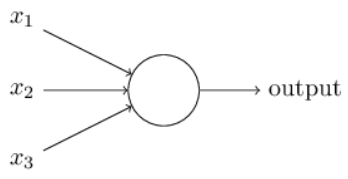
\includegraphics[width=0.5\textwidth]{docu_img_01}
    \caption{Perzeptron}
    \label{fig:perzeptron}
\end{figure}

Im gezeigten Bild ist beispielsweise ein Neuron dargestellt, das drei Inputgrößen akzeptiert und daraus einen Output produziert. Um den Output zu berechnen werden Gewichte (\textit{engl. weights}) eingeführt. Ob das Neuron 0 oder 1 als Output liefert, hängt dann davon ab, ob die gewichtete Summe der Eingangsgrößen einen zu definierenden Schwellwert überschreitet.

Dies kann anhand der nachfolgenden Formel verdeutlicht werden:

\begin{figure}[H]
    \centering
    \[ output =
      \begin{cases}
        0 \quad \text{if } \sum \omega_i x_i \leqslant \text{ threshold (Schwellwert)}\\
        1 \quad \text{if } \sum \omega_i x_i > \text{ threshold (Schwellwert)}
      \end{cases}
    \]
    \caption{Berechnung des Outputs.}
    \label{fig:neuron-three-way}
\end{figure}

Dies ist das grundlegende Modell. Grundsätzlich kann sich das Perzeptron auch als ein ``Entscheidungs-Unterstützer'' vorstellt werden, der eine Entscheidung trifft, in dem er konkrete Fakten mit einem bestimmten Gewicht versieht.

Das gezeigte Modell ist augenscheinlich sehr simpel und noch sehr weit von dem entfernt, was als ein neuronales Netz bezeichnet werden würde. Es ist allerdings ohne Weiteres denkbar, das gezeigte Model komplexer zu gestalten, indem mehrere Perzeptrons miteinander verknüpft werden, so dass beispielsweise das nachfolgende Netzwerk entstehen könnte:

\begin{figure}[H]
    \centering
    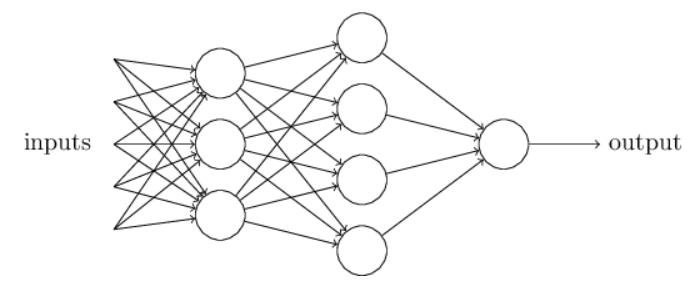
\includegraphics[width=0.5\textwidth]{docu_img_03}
    \caption{Mehrschichtiges neuronales Netz.}
    \label{fig:multi-layer-net}
\end{figure}

In Grafik\textsuperscript{\ref{fig:neuron-three-way}} wurde ein Schwellwert eingeführt, der überschritten werden muss, damit ein Perzeptron aktiviert wird. Um das Modell zu vereinheitlichen, kann der \textit{Bias} definiert werden, der den negativen Schwellwert darstellt. Durch diese Maßnahme kann die Aktivierungsfunktion des Perzeptrons dann geschrieben werden als:

\begin{figure}[H]
    \centering
    \[ output =
          \begin{dcases}
            0 \quad \text{if } \sum \omega \cdot x + b \leq 0 \\
            1 \quad \text{if } \sum \omega \cdot x + b > 0
          \end{dcases}
    \]
    \caption{Berechnung des Outputs bei Verwendung eines Bias.}
    \label{fig:bias-calculation}
\end{figure}

Inhaltlich kann der Bias als ein Maß verstanden werden, aus dem hervorgeht, wie \textit{leicht} ein Perzeptron aktiviert werden kann. Nimmt der Bias einen großen Wert an, so kann das Perzeptron einen Wert von 1 annehmen, auch wenn das Produkt aus den Gewichten und den Eingangsgrößen einen negativen Wert annimmt. Gleiches gilt selbstverständlich auch für einen kleinen Bias, der zur Folge hat, dass ein Perzeptron träger reagiert.

NOTE:
wiederholung gehirn menschlich lernen

\subsection{Sigmoid-Neuronen}

Eine Weiterentwicklung des zuvor vorgestellten Modells stellen Sigmoid-Neuronen dar. Diese Weiterentwicklung wird dann erforderlich, wenn das Anpassen der Gewichte - also letztlich das Lernen - betrachtet wird. Dabei ist das Ziel, dass eine kleine Anpassung eines Gewichts auch nur eine kleine Änderung des Outputs zur Folge hat. Das zuvor betrachtete Perzeptron ist lediglich in der Lage 0 oder 1 als Output zu liefern, so dass Änderungen an den Gewichten keine stetige Änderung des Outputs zur Folge haben, sondern folgenlos bleiben können bis irgendwann ein Sprung von 0 auf 1 oder umgekehrt stattfindet, was wiederum eine große Änderung darstellt.

Die Weiterentwicklung besteht nun in einer Verfeinerung der Aktivierungsfunktion. Anstatt eine Sprungfunktion\textsuperscript{\ref{fig:step-function}} zu verwenden, die lediglich 0 und 1 als Funktionswert annehmen kann, wird die Sigmoid Funktion\textsuperscript{\ref{fig:sigmoid-function}} eingeführt, die die folgende Form hat:

\begin{figure}[H]
    \centering
    \[ \sigma(z) \equiv
          \frac{1}{1+e^{-z}}
    \]
    \caption{Sigmoid-Funktion.}
    \label{fig:sigmoid}
\end{figure}

Der entscheidende Unterschied kann an den beiden nachfolgenden Grafiken verdeutlicht werden, die jeweils die Kurve der entsprechenden Funktion darstellen:

\captionsetup[subfigure]{labelformat=empty, labelsep=none}
\begin{figure}[H]
    \centering
    \begin{subfigure}{0.45\textwidth}
		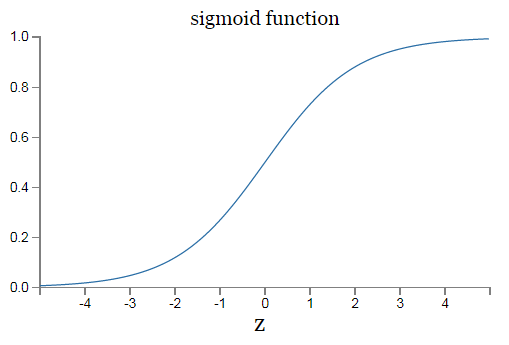
\includegraphics[width=0.9\textwidth]{docu_img_06}
		\caption{\tiny{Sigmoid Funktion.}}
		\label{fig:sigmoid-function}
	\end{subfigure}
    \begin{subfigure}{0.45\textwidth}
		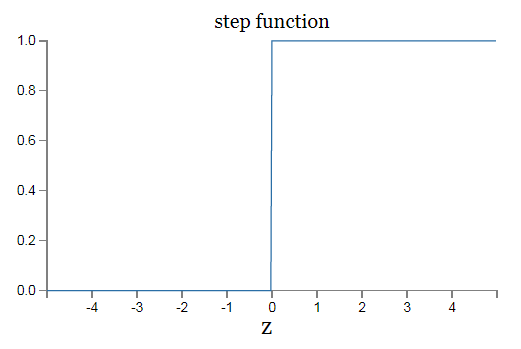
\includegraphics[width=0.9\textwidth]{docu_img_07}
		\caption{\tiny{Step Funktion.}}
		\label{fig:step-function}
	\end{subfigure}

    \caption{Vergleich der Aktivierungsfunktionen \textit{Sigmoid} und \textit{Step-Funktion}}
    \label{fig:activation-functions}
\end{figure}

\subsection{Architektur neuronaler Netze}

Mit diesen Bestandteilen als Ausgangspunkt können nun tatsächlich konkretere Neuronale Netze und deren Architekturen eingeführt werden. Neuronale Netze bestehen üblicherweise aus mehreren Schichten, den \textit{Layern}. Diese lassen sich grundsätzlich in drei Kategorien aufteilen: Input, Hidden und Output. Neuronale Netze beinhalten für gewöhnlich ein Input-Layer und ein Output-Layer sowie dazwischen beliebig viele Hidden-Layer. Die Form der Input- und Output-Layer ist dabei sehr naheliegend: das Input-Layer hat die gleiche Struktur wie die des Inputs und das Output-Layer hat entsprechend die gleiche Struktur wie der Output.

Angenommen es sollen Bilder der Größe 28 \(\times\) 28 Pixel klassifiziert werden und es gibt 10 mögliche Klassen, dann besteht das Input-Layer aus 28 \(\times\) 28 = 784 Neuronen und das Output-Layer aus 10 Neuronen.

Lediglich der Bereich zwischen Input- und Output-Layer - die Hidden-Layer - lässt sich nicht ohne Weiteres aus dem Input oder dem Output ableiten. Es gibt lediglich Heuristiken, die beim Design der Hidden-Layer angewandt werden können, allerdings keine konkreten Regeln, die befolgt werden müssen. Diese Struktur kann anhand des nachfolgenden Bilds verdeutlicht werden, bei dem - um die Übersichtlichkeit zu wahren - das Input-Layer etwas komprimiert dargestellt wird:

NOTES:
pyton tutorial uh - > softcomputing

\begin{figure}[H]
    \centering
    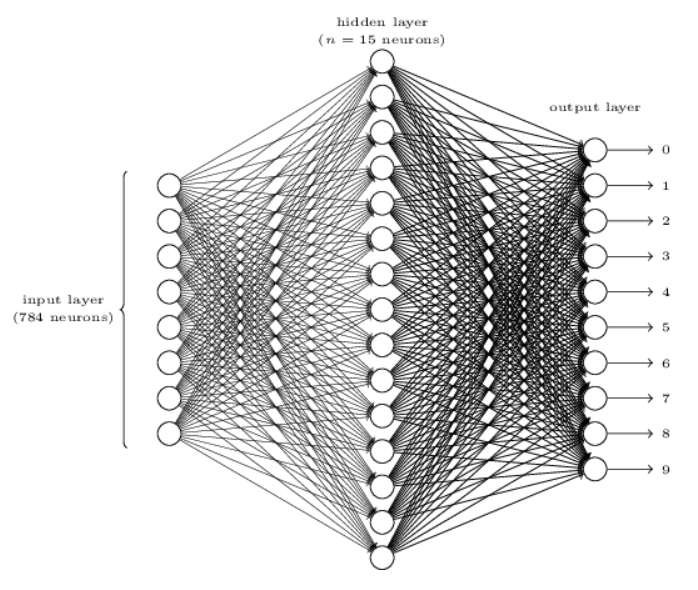
\includegraphics[width=0.9\textwidth]{docu_img_08}
    \caption{Hidden-Layer Darstellung.}
    \label{fig:hidden-layers}
\end{figure}

\subsection{Lernen - Das Anpassen der Gewichte}

Das Lernen stellt den zentralen Ansatz von neuronalen Netzes dar. Eng im Zusammenhang mit dem Lernen steht eine
Kosten-Funktion, die häufig auch als Verlust-Funktion bezeichnet werden kann. Diese stellt letztlich den Fehler zwischen
dem Erwartungswert und dem tatsächlichen Wert, den das neuronale Netz berechnet, dar. Mathematisch betrachtet ist das
grundlegende Prinzip des Lernens, diese Funktion zu minimieren, also zu gewährleisten, dass die Abweichungen zwischen
Erwartungswert und tatsächlichem Wert möglichst gering sind. Es sind grundsätzlich viele verschiedene Verlust-Funktionen
denkbar, eine, die jedoch eine breite Verwendeung findet, ist die quadratische Kosten-Funktion - auch als \textit{mean squared
error} (MSE) bezeichnet.

\begin{figure}[H]
    \centering
    \[ C(w, b) \equiv
          \frac{1}{2n}\displaystyle\sum_{x}{\parallel y(x) - a\parallel^2}
    \]
    \caption{Mean Squared Error (MSE).}
    \label{fig:learn-function}
\end{figure}

Dabei beschreiben \textit{w} und \textit{b} die Gewichte bzw. die Bias des neuronalen Netzes und \textit{n} stellt die Anzahl der Trainingsdaten
dar. Der Vektor a beschreibt den Output des Netzes und \textit{\(y(x)\)} stellt den Erwartungswert zu einem Input \textit{x} dar.
Das Ziel besteht nun darin, die Gewichte und Bias so zu manipulieren, dass die gezeigte Funktion einen möglichst kleinen
Wert annimmt.







--
Wie Neuronen funktionieren
Die Arbeitsweise ist erstaunlich einfach:
Immer wenn die Summe der Eingangssignale einen bestimmten Schwellenwert überschreitet,
sendet die Zelle ein Ausgangssignal.
Bleibt die Eingangserregung unter der Grenze, reagiert die Zelle nicht.
Am Ende der axonalen Verzweigungen stellt eine besondere Struktur, die Synapse,
den Kontakt zu anderen Neuronen her.
Die meisten Synapsen funktionieren so:
Je stärker die Erregung im Axon, desto mehr Moleküle einer Überträgersubstanz
schüttet die Synapse aus. Der Überträgerstoff (Neurotransmitter) wandert zur Zielzelle.
Manche Neurotransmitter erhöhen die elektrische Erregung der "angefunkten" Zelle,
andere hemmen sie. 

Die Netzwerke der Erinnerung
Das Netzwerk der Neuronen in der Großhirnrinde (wegen ihrer Form auch „Pyramidenzellen“)
ist im Gegensatz zu einem Computer nicht nach einem detaillierten Plan geknüpft,
sondern weitgehend zufällig organisiert.
Sind miteinander verbundene Zellen gemeinsam aktiv, verstärken sich die Synapsen.
Demnach aktiviert das Lernen immer wieder eine Anzahl miteinander verknüpfter
Pyramidenzellen. Deren Verbindung verstärkt sich nach und nach,
„neuronale Netzwerke“ entstehen.
Je öfter sich der synaptische Lernprozess wiederholt, desto leichter
lässt sich dieses „Netzwerk“ aktivieren. 
--

\subsection{Arten und Anwendungsgebiete}

es gibt sie in allen formen und farben. nns zu listen, wäre ein akt der unmöglcihekit. 
im netz finden sich links wie:

The mostly complete chart of Neural Networks, explained
https://towardsdatascience.com/the-mostly-complete-chart-of-neural-networks-explained-3fb6f2367464

und
liste auf wikipedia
https://en.wikipedia.org/wiki/Types\_of\_artificial\_neural\_networks


\subsection{Überwachtes und Unüberwachtes Lernen}
Lorem ipsum dolor sit amet, consetetur sadipscing elitr, sed diam nonumy eirmod tempor invidunt ut labore et dolore magna aliquyam erat, sed diam voluptua. At vero eos et accusam et justo duo dolores et ea rebum. Stet clita kasd gubergren, no sea takimata sanctus est Lorem ipsum dolor sit amet. Lorem ipsum dolor sit amet, consetetur sadipscing elitr, sed diam nonumy eirmod tempor invidunt ut labore et dolore magna aliquyam erat, sed diam voluptua. At vero eos et accusam et justo duo dolores et ea rebum. Stet clita kasd gubergren, no sea takimata sanctus est Lorem ipsum dolor sit amet.

